\documentclass[../DS08.tex]{subfiles}%
\graphicspath{{./figures/}}%

% \subimport{/home/nora/Documents/Enseignement/Prepa/bpep/exercices/TD/autour_E-pH_du_chlore/}{sujet.tex}%

\begin{document}%
\prblm[53]{Exploitation du diagramme $E-\pH$ du chlore\ifcorrige{~\small\textit{(D'après
			Centrale TSI 2018)}}}%

\subsection{Diagramme du chlore}%

\enonce{%
La figure~\ref{fig:E-pHCl} donne le diagramme potentiel$-\pH$ de
l'élément chlore. Les espèces considérées, qui sont toutes en solution, sont
$\ce{Cl2_(aq)}$, $\ce{Cl^-_{(aq)}}$, $\ce{ HClO_{(aq)}}$ et $\ce{ClO^-_{(aq)}}$.
La concentration de tracé est $c = \SI{1,0e-1}{ \mol \per\liter}$. Les
frontières entre deux espèces ont été calculées en traduisant l'égalité des
\emph{concentrations molaires en élément} chlore de chaque espèce sur la
frontière, la somme de ces concentrations étant égale à $c$.
\begin{figure}[h]
	\centering
	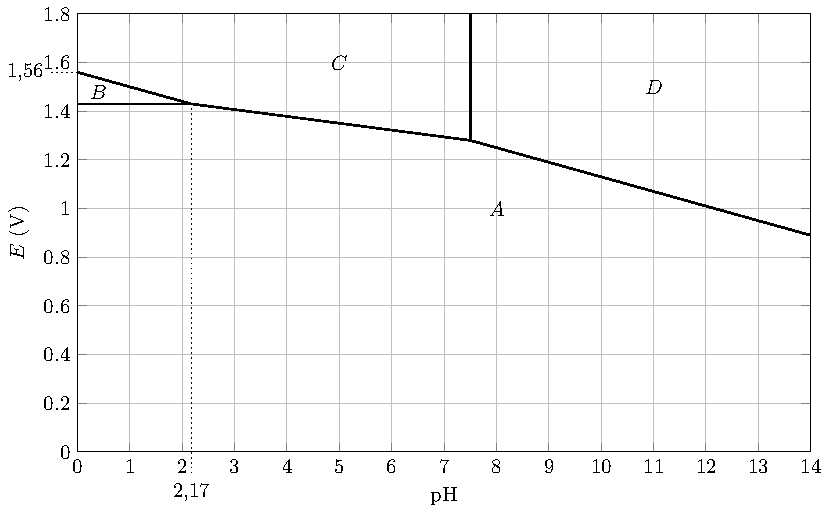
\includegraphics[scale=.9]{eph_chlore}
	\caption{Diagramme E-pH du chlore}%
	\label{fig:E-pHCl}%
\end{figure}%
}%

\QR[7]{%
Justifier que les espèces $A$, $B$, $C$ et $D$ sont respectivement
$\ce{Cl^-_{(aq)}}$, $\ce{Cl_{2\,(aq)}}$, $\ce{HClO_{(aq)}}$ et
$\ce{ClO^-_{(aq)}}$.
}{%
~
\smallbreak
\vspace*{-25pt}
\noindent
\begin{minipage}[c]{.60\linewidth}
	\begin{center}
		\captionof{table}{Calcul du nombre d'oxydation}
		\begin{tabularx}{\linewidth}{cYYYY}
			\toprule
			Espèce                &
			$\ce{HClO_{\aqu}}$    &
			$\ce{{ClO}^-_{\aqu}}$ &
			$\ce{{Cl_2}_{\aqu}}$  &
			$\ce{{Cl}^-_{\aqu}}$
			\\
			\no{Cl}               &
			$+\myRoman{1}$ \pt{1} &
			$+\myRoman{1}$        &
			0            \pt{1}   &
			$-\myRoman{1}$ \pt{1}
			\\
			Domaine \pt{1}        &
			C                     & D & B & A
			\\
			\bottomrule
		\end{tabularx}
	\end{center}
\end{minipage}
\hfill
\begin{minipage}[c]{.39\linewidth}
	\vspace*{0pt}
	\begin{center}
		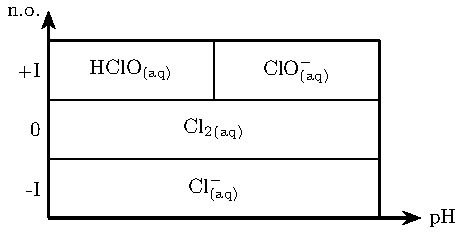
\includegraphics[width=\linewidth]{esit_chlore}
		\captionof{figure}{Diagramme de situation\protect\pt{1}+\protect\pt{1}}
	\end{center}
\end{minipage}
\smallbreak
On prouve le caractère acide de \ce{HClO} par une équation~:
\[
	\ce{HClO_{\aqu} + H_2O_{\liq} \stm{=} {ClO}^-_{\aqu} + {H_3O}^+_{\aqu}}
	\tag*{$K_A$}
\]
}%

\QR[3]{%
	Déterminer le $\pk$ du couple $\ce{HClO / ClO^-}$.
}{%
	Pour des espèces acido-basiques dissoutes, par la relation de \textsc{Henderson}
	on a
	\[
		\pH \stm{=} \pk + \log \frac{[\ce{HClO}]}{[\ce{ClO^-}]}
		\Ra
		\boxed{\pH\ind{front} \stm{=} \pk}
		\Ra
		\xul{\pk \stm{=} \num{7.25}}
	\]
}%

\QR[7]{%
Déterminer le potentiel standard du couple $B/A$.
}{%
La demi équation rédox du couple \ce{B/A} est $\ce{{Cl_2}_{\aqu} + 2 e-
	\stm{=} 2 Cl^-_{\aqu}}$, ainsi l'équation de la frontière est donnée par
\[
	E \stm{=} E^\circ + \frac{\num{0,06}}{2}\log \frac{[\ce{Cl2}]c^\circ}{[\ce{Cl^-}]^2 }
\]
On nous signale qu'il y a  égalité des concentrations en  éléments sur la
frontière, donc $2[\ce{Cl2}] = [\ce{Cl^-}]$, et comme $2[\ce{Cl2}] +
	[\ce{Cl^-}] = c$, nous avons que $[\ce{Cl2}] = c/4$ et $[\ce{Cl^-}] = c/2$.
Finalement
\[
	\boxed{E \stm{=} E^\circ  - \num{0, 03} \log c}
\]
Pour déterminer $E$ on peut utiliser les informations sur la frontière entre $B$
et $C$:
\[
	\ce{2 HClO_{\aqu} + 2 H^+_{\aqu} + 2 e^- \stm{=} {Cl_2}_{\aqu} + 2 H2O_{\liq}}
\]
ainsi la pente est de \SI{0,06}{\volt\per pH}, et ainsi
\[
	E = \SI{1,56}{\volt} -
	\SI{0,06}{\volt\per pH} \cdot \SI{2, 17}{pH} \stm{=} \SI{1, 43}{\volt}
\]
En conclusion,
\[
	\boxed{E^\circ \stm{=} E + \num{0,03} \log c}
	\Ra \xul{E^\circ \stm{=} \SI{1,40}{ V}}
\]
}%

\QR[2]{%
Écrire la demi-équation redox entre les espèces $A$ et $C$.
}{%
\leavevmode\vspace*{-15pt}\relax
\[
	\ce{HClO_{\aqu} + H^+_{\aqu} + 2 e^- \stm{\stm(un){=}} Cl^-_{\aqu} + H2O_{\liq}}
\]
}%

\QR[3]{%
	Déterminer la pente de la frontière $C/A$ et en effectuer la vérification
	graphique.
}{%
	La formule de \textsc{Nernst} pour ce couple donne
	\[
		E \stm{=} E^\circ + \num{0,03}
		\log \frac{[\ce{HClO}][\ce{H^+}]}{[\ce{Cl^-}]}
		\Lra
		E\ind{front} \stm{=} E^\circ - \SI{0,03}{pH}
	\]
	Avec l'égalité des concentrations à la frontière. Ainsi, la pente est de
	\SI{-0,03}{\volt\per pH} \pt{1}. En prolongeant la frontière, on remarque
	qu'elle passe par les points $(2, 17 ;1,43)$ et $(10,5 ;1,2)$, ce qui confirme
	une pente de \SI{-0, 03}{\volt\per pH} \pt{1}.
}%

\QR[2]{%
	Déterminer le potentiel standard du couple $C/A$.
}{%
	En $\pH = \num{2,17}$, $E \stm{=} \SI{1,43}{\volt}$, ainsi $E^\circ  = \SI{1,
			43}{V} + \SI{0, 03}{\volt\per pH} \cdot \SI{2.17}{pH} \stm{=} \SI{1,50}{V}$
}%

\subsection{Diagramme de l'eau}%

\enonce{%
	On considère les espèces $\ce{H2O}$, $\ce{O2_{(g)}}$ et $\ce{ H2_{(g)}}$. La
	pression de tracé est fixée à \SI{1}{ \bar} et la concentration de tracé à
	\SI{1,0}{\mol\per\liter}.
}%

\QR[8]{%
	Déterminer les équations des frontières.
}{%
	On écrit les demi-équations associées puis les potentiels~:
	\begin{itemize}
		\item $\ce{O2_{\rm(g)}/H_2O_{\rm(l)}}$~: \pt{1}
		      \vspace{-20pt}
		      \begin{gather*}
			      \ce{
			      2 {H_2O}_{\rm(l)}
			      \stm{=}
			      {O_2}_{\rm(g)} + 4 {H}^+_{\rm(aq)} +4 e^-
			      }
			      \\\Ra
			      E_1 \stm{=}
			      E_1^\circ + \frac{\num{0.06}}{4} \log (\frac{[\ce{H+}]^4
				      p_{\ce{O_2}}}{{c^\circ}^4 p^\circ})
			      \\\Lra
			      E_1 =
			      E_1^\circ - \num{0.06}\pH + \num{0.06}\log (\frac{p_{\ce{O_2}}}{p^\circ})
			      \\\Ra
			      \beforetext{$p\ind{\ce{O_2},front} = \SI{1}{bar} = p^\circ$}
			      \boxed{E\ind{1,front} \stm{=} E_1^\circ - \num{0.06}\pH}
		      \end{gather*}
		\item $\ce{H_2O_{\rm(l)}/H_2{\rm(g)}}$~: \pt{1}
		      \vspace{-20pt}
		      \begin{gather*}
			      \ce{
			      {H_2}_{\rm(g)}
			      \stm{=}
			      2H^+_{\rm(aq)} + 2e^-
			      }
			      \\\Ra
			      E_2 \stm{=}
			      E_2^\circ + \frac{\num{0.06}}{2} \log (\frac{[\ce{H^+}]^2
				      p^\circ}{{c^\circ}^2 p_{\ce{H_2}}})
			      \\\Lra
			      E_2 =
			      E_2^\circ - \num{0.06}\pH + \num{0.06}\log (\frac{p^\circ}{p_{\ce{H_2}}})
			      \\\Ra
			      \beforetext{$p\ind{\ce{O_2},front} = \SI{1}{bar} = p^\circ$}
			      \boxed{E\ind{2,front} \stm{=} E_2^\circ - \num{0.06}\pH}
		      \end{gather*}
	\end{itemize}
}%

\QR[4]{%
	Tracer succinctement sur votre copie l'allure du diagramme potentiel$-\pH$ de
	l'eau superposé à celui du chlore aqueux. Quels commentaires pouvez-vous
	formuler ?
}{%
	les lignes de séparation des domaines de l'eau partent à pH=0 à 0 et
	\SI{1,23}{V} respectivement, avec une pente de \SI{-,06}{\volt\per pH} \pt{1},
	elles sont \textbf{intégralement en dessous} \pt{1} de tous les autres
	segments du diagramme E-pH. En superposant ces deux diagrammes, nous
	remarquons que seul \ce{Cl^-} peut coexister \pt{1} dans l'eau car toutes les
	autres espèces ont des domaines disjoints \pt{1} avec celui de l'eau.
}%

\subsection{Étude de la cellule d'électrolyse}%
\enonce{%
	\begin{minipage}{.48\columnwidth}%
		\begin{center}%
			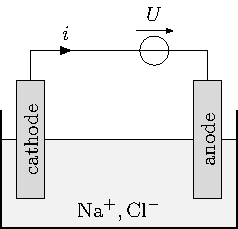
\includegraphics[scale=1]{electrolyse}
			\captionof{figure}{L'électrolyseur}%
			\label{fig:électrolyseur}%
		\end{center}%
	\end{minipage}%
	\begin{minipage}{.5\columnwidth}%
		L'électrolyseur est constitué de deux électrodes en titane. Il force la
		réaction inverse de la réaction spontanée. Le schéma de principe est donné
		figure~\ref{fig:électrolyseur}. La tension $U$ et le courant $i$ sont donc des
		grandeurs positives, mais la nature chimique de l'anode et de la cathode sont
		inchangées. Lors de la mise sous tension de l'électrolyseur, on observe une
		production de $\ce{ H2_{(g)}}$ et de $\ce{Cl2_{(aq)}}$. L'électrolyseur est
		placé en amont du système de filtrage de l'eau.
	\end{minipage}%
}%

\QR[4]{%
Écrire les demi-réactions électroniques des réactions se déroulant à l'anode
et à la cathode.
}{%
À l'anode il se produit une \textbf{oxydation} \pt{1}, ainsi il se produit du
\ce{Cl2} selon la réaction $\ce{2 Cl^-_{\aqu} \stm{=} {Cl2}_{\aqu} + 2 e^-}$.
\smallbreak
À la cathode, il se produit une \textbf{réduction} \pt{1}, donc la formation
de \ce{H2} selon la réaction $\ce{2 H^+_{\aqu} + 2 e^- \stm{=} {H2}_{\gaz}}$
}%

\enonce{
	L'eau d'une piscine est maintenue à un $\pH$ compris entre \num{7,0} et \num{7,4}.
}%

\QR[4]{%
Écrire l'équation modélisant la réaction chimique qui, à partir de
$\ce{Cl2_{(aq)}}$ en solution aqueuse, forme $\ce{Cl^-_{(aq)}}$ et
$\ce{ClO^-_{(aq)}}$. Comment s'appelle ce type de réaction~?
}{%
\leavevmode\vspace*{-15pt}\relax
\begin{gather*}
	\ce{{Cl2}_{\aqu} + 2 e^- \stm{=} 2 Cl^-_{\aqu}}%
	\\
	\ce{{Cl2}_{\aqu} + 2 H2O_{\liq} \stm{=} 2 ClO^-_{\aqu} + 4 H^+_{\aqu} + 2 e^-}
	\\\Ra
	\ce{ {Cl2}_{\aqu} + H2O_{\liq} \stm{=} Cl^-_{\aqu} + ClO^-_{\aqu} + 2 H^+_{\aqu}}
\end{gather*}
C'est une \textbf{dismutation}. \pt{1}
}%

\enonce{%
	On envisage dans la suite une piscine d'um particuliær de contenance
	$V_0 = \SI{150}{\cubic\meter}$.
}%

\QR[2]{%
	Avant la mise en fonctionnement de l'électrolyseur, l'eau de la piscine doit
	être salée avec une teneur en sel d'environ $c_s = \SI{5}{\gram\per\liter}$
	(on prendra cette valeur pour les applications numériques). Quelle masse de
	sel læ particuliær doit-iel acheter lors de la première mise en route du
	dispositif~?
}{%
	\leavevmode\vspace*{-15pt}\relax
	\[
		m \stm{=} c_s\cdot V_0 = \SI{5}{\gram\per\litre} \cdot \SI{150}{\cubic\meter}
		\stm{=} \SI{750}{kg}
	\]
}%

\enonce{
	Un fabricant d'électrolyseurs de piscines annonce, pour un modèle
	adapté à un volume maximal de bassin de \SI{150}{\cubic\meter}, une
	production horaire maximale $\dv{m\ind{max}}{t} = \SI{26}{\gram\per \hour}$
	de $\ce{Cl2}$. Pour ce modèle, $U = \SI{7,5}{\volt}$.
}%

\QR[4]{%
	Calculer la valeur de $i$ correspondant au fonctionnement maximal. On
	supposera le fonctionnement idéal.
}{%
	Cherchons la quantité de dichlore formée par seconde~:
	\[
		n_{\ce{Cl2}} \stm{=} \frac{m\ind{max}}{2 M_{\ce{Cl}}\times\SI{3600}{\second\per\hour}}
	\]
	Or la formation à l'anode d'une mole de \ce{Cl2} s'accompagne de la libération
	de 2 moles d'électrons, ainsi $n_e \stm{=} 2 n_{\ce{Cl2}}$. Finalement,
	\[
		\boxed{i \stm{=} e \mathcal N_a \frac{n_e}{\Delta{t}} =
			\mathcal{F}
			\frac{m_{\text{max}}}{M_{\ce{Cl}}\times\SI{3600}{\second\per\hour}} \stm{=}
			\SI{20}{A}}
	\]
}%

\QR[3]{%
	Calculer la puissance correspondant à une production horaire maximale.
	Commenter le résultat.
}{%
	$P \stm{=} U I \stm{=} \SI{150}{W}$, ce qui n'est pas excessif, sauf s'il faut
	la faire tourner en continu… \pt{1}
}%

\end{document}%
